\chapter{Data acquisition for CHIPS} %%%%%%%%%%%%%%%%%%%%%%%%%%%%%%%%%%%%%%%%%%%%%%%%%%%%%%%%%%%%%
\label{chap:daq} %%%%%%%%%%%%%%%%%%%%%%%%%%%%%%%%%%%%%%%%%%%%%%%%%%%%%%%%%%%%%%%%%%%%%%%%%%%%%%%%%

The primary task of any Data Acquisition (DAQ) system is the processing of low-level signals
measuring real-world physics and their transfer to permanent storage for further analysis.
Commonly, this procedure also includes decision making as to whether the signal is deemed
interesting enough to record, known as a \emph{trigger}. These tasks can make DAQ systems
incredibly complex, especially when they must operate in an efficient and resilient manner for
vast amounts of data in real-time, while also providing detector control and monitoring.

In the context of the \chips project, the DAQ system records all PMT hits, timestamps them using a
common clock, and transfers them out of the detector to a central processing node. This node then
applies a trigger to select hits that fall within the interesting beam spill time window. All
selected hits are sliced into events and moved to permanent storage for further analysis.
Alongside these processes, the DAQ also configures the detector and provides data quality and
detector component monitoring.

Although relatively simple when compared to the complex and time-pressured DAQ systems of the LHC
experiments, the DAQ system developed for the \chips project introduces some novel approaches to
solve the unique constraints of the \chips concept. Namely, deployment within a body of water and
a limited resource budget. In this chapter, the DAQ implementation for \chips as applied to the
\chipsfive prototype detector module is described alongside highlighting these novel approaches.
The description is presented in two broad categories, hardware and software, with a short
description of the timing system to begin.

\section{White Rabbit timing} %%%%%%%%%%%%%%%%%%%%%%%%%%%%%%%%%%%%%%%%%%%%%%%%%%%%%%%%%%%%%%%%%%%%
\label{sec:daq_timing} %%%%%%%%%%%%%%%%%%%%%%%%%%%%%%%%%%%%%%%%%%%%%%%%%%%%%%%%%%%%%%%%%%%%%%%%%%%

To ensure PMT hit times are synchronised throughout \chips detectors, a common clock must be
shared across all timestamping electronics. For this purpose \chips employs a \emph{White Rabbit}
(WR) network~\cite{lipinski2011}. Initially developed at CERN, the open-source WR project provides
an ethernet-based time distribution network with sub-nanosecond synchronisation accuracy between
nodes. By using many two-way exchanges of WR messages, precise adjustment of individual clock
phases and offsets is possible across thousands of nodes, separated by tens of kilometres. All of
this is achieved in parallel with a standard data transfer network capable of
\unit{1}{\mathrm{Gb}} speeds.

All nodes are synchronised to the clock of a \emph{GrandMaster} node which is typically a WR
\emph{switch}, the most common WR hardware component. As input, this switch receives a Pulse Per
Second (PPS) and \unit{10}{\mathrm{MHz}} signal from a GPS disciplined oscillator. When used in
conjunction with a Network Time Protocol (NTP) server connection, these inputs allow for the WR
network to be synchronised to International Atomic Time (TAI). This timing is particularly
important for \chips detector modules which require synchronisation to accelerator clocks many
hundreds of kilometres away (such as the Fermilab Main Injector clock) in order to determine the
arrival time of beam spills accurately.

WR hardware is commercially available from many vendors. Within \chipsfive two WR devices are used
for time synchronisation and data transfer, both shown in Fig.~\ref{fig:wr_electronics}. Firstly,
a compact version of the standard WR switch~\cite{wrswitch2020}, specially developed for the
\chips project at Nikhef~\cite{wrchromium2020}. Secondly, a WR Lite Embedded Node (LEN) from Seven
Solutions~\cite{wrlen2020}. All WR components are connected using \unit{1}{\mathrm{Gb}}
bi-directional optical fibre connections using the \unit{1310}{\mathrm{nm}} and
\unit{1550}{\mathrm{nm}} wavelengths via Small Form-Factor Pluggable Transceivers (SFPs).

\begin{figure} % WHITE-RABBIT COMPONENTS DIAGRAM %
    \centering
    \subcaptionbox{White Rabbit switch}{%
        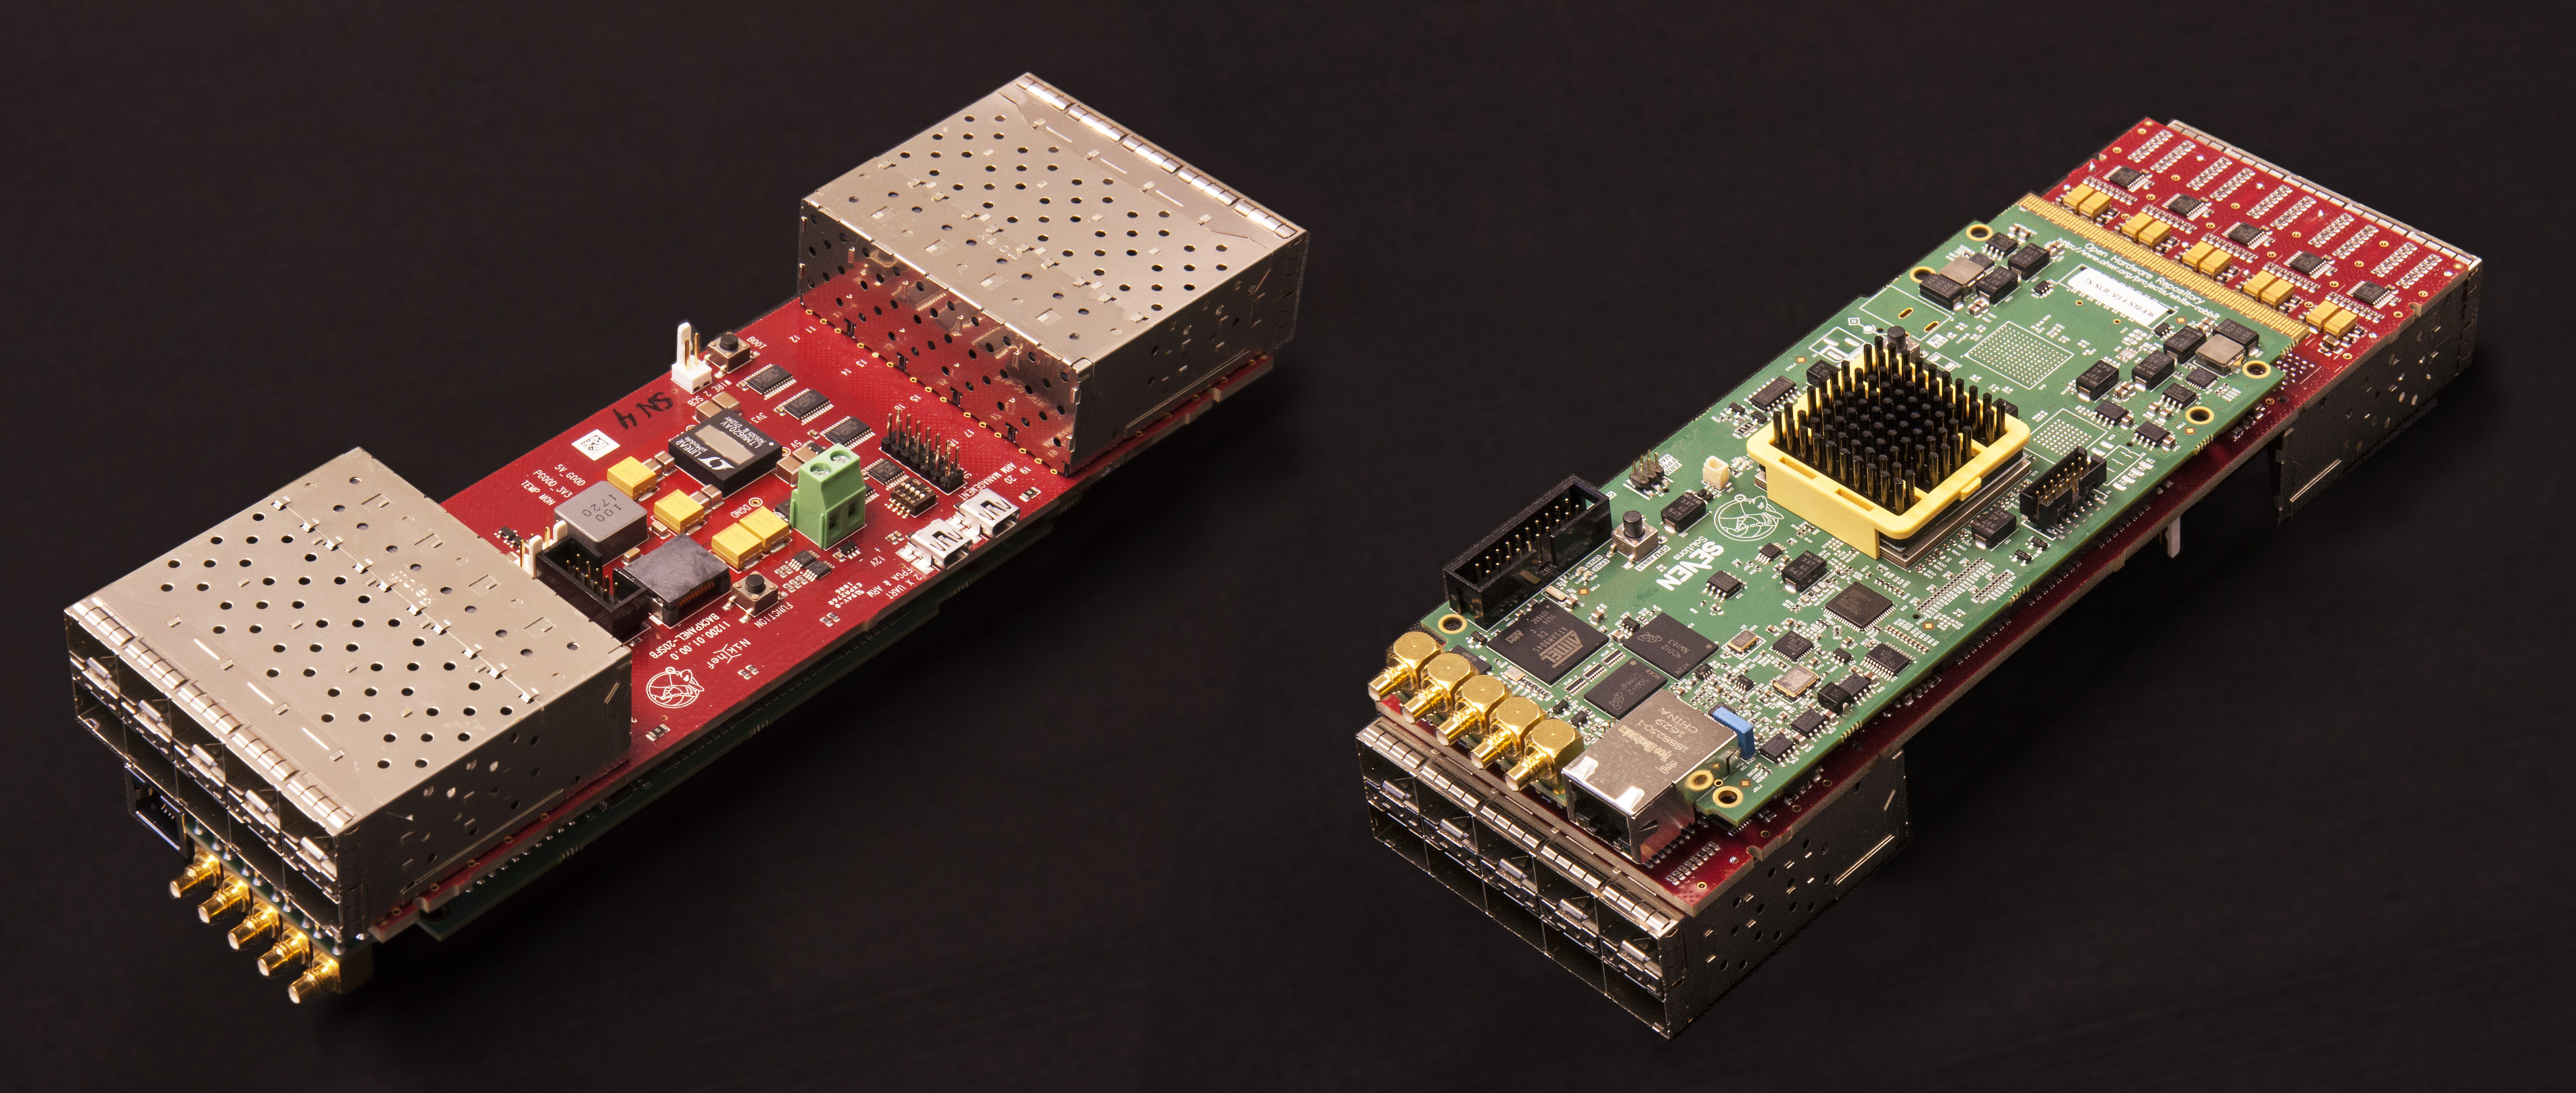
\includegraphics[height=6cm]{diagrams/5-daq/wr_switch.jpg}%
    }
    \quad
    \subcaptionbox{White Rabbit LEN}{%
        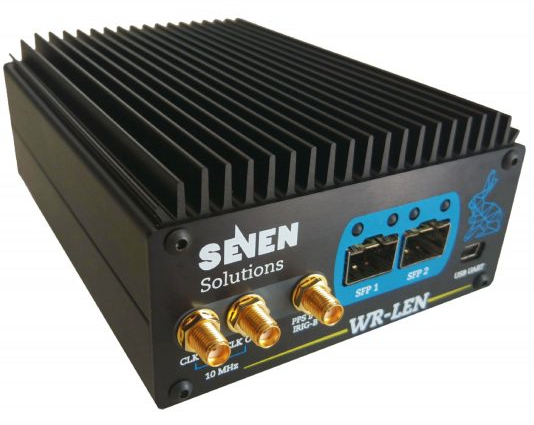
\includegraphics[height=6cm]{diagrams/5-daq/wr_len.jpg}%
    }
    \caption[Pictures of the White Rabbit timing hardware used within \chipsfive.]
    {Pictures of the White Rabbit timing hardware used within \chipsfive. The compact White rabbit
        switch specially designed for \chips is shown in (a), while the White Rabbit Lite Embedded
        Node (LEN) from Seven Solutions is shown in (b).}
    \label{fig:wr_electronics}
\end{figure}

Fig.~\ref{fig:sync} shows the WR synchronised PPS clock rising edges for two WR switches used
within \chipsfive separated by \unit{500}{\mathrm{m}} of fibre. With the vertical ticks
representing single nanoseconds, sub-nanosecond time synchronisation accuracy is achieved.

\begin{figure} % WHITE-RABBIT SYNC DIAGRAM %
    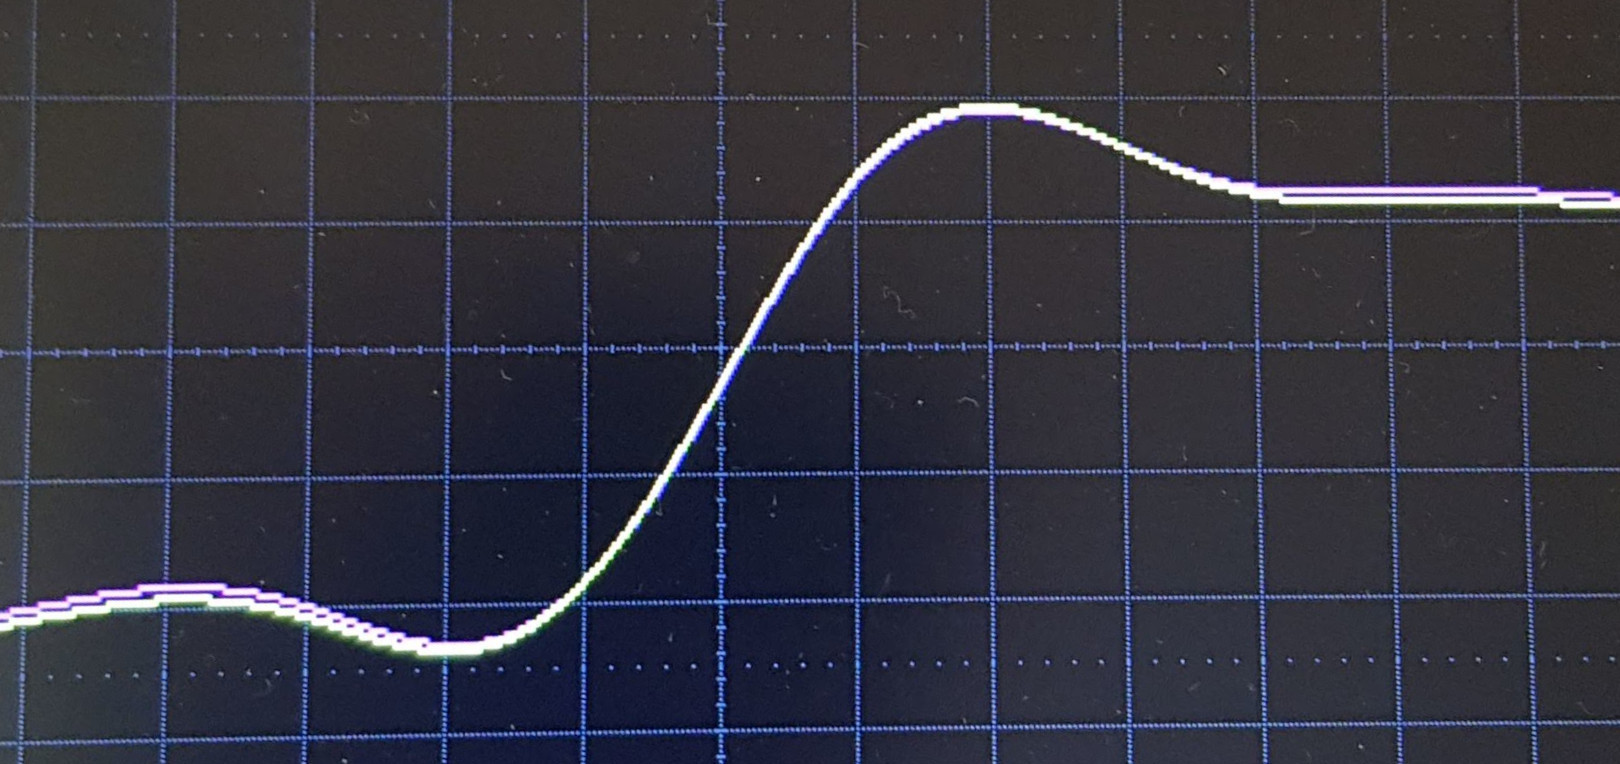
\includegraphics[width=0.7\textwidth]{diagrams/5-daq/sync.jpg}
    \caption[Picture of White Rabbit timing synchronisation seen in \chips.]
    {Picture of an oscilloscope measuring the PPS output signal of two WR switches shown in pink
        and yellow at either end of a \unit{500}{\mathrm{m}} long optical fibre. The vertical
        ticks are in nanoseconds showing the sub-nanosecond synchronisation possible with the WR
        timing network.}
    \label{fig:sync}
\end{figure}

\section{Hardware} %%%%%%%%%%%%%%%%%%%%%%%%%%%%%%%%%%%%%%%%%%%%%%%%%%%%%%%%%%%%%%%%%%%%%%%%%%%%%%%
\label{sec:daq_hard} %%%%%%%%%%%%%%%%%%%%%%%%%%%%%%%%%%%%%%%%%%%%%%%%%%%%%%%%%%%%%%%%%%%%%%%%%%%%%

The hardware of the \chipsfive DAQ system is split into two distinct implementations at its lower
levels (closest to the PMTs), corresponding to the Nikhef and Madison POM types. \chips R\&D
efforts have developed the novel Madison implementation with the view to use this hardware within
detector modules exclusively. However, as a safe stepping stone, while development and testing are
still ongoing, \chipsfive mainly contains proven Nikhef hardware developed for the KM3NeT
experiment~\cite{adrian2016}.

The complete DAQ and power distribution system for \chipsfive is shown in Fig.~\ref{fig:daq}. The
following subsections describe each component starting from the lowest level and working upwards.
The Nikhef and Madison descriptions are separated for clarity as well as the high-level combined
hardware systems, part of which is not located within the detector but onshore in an electronics
hut.

\begin{figure} % DAQ DIAGRAM %
    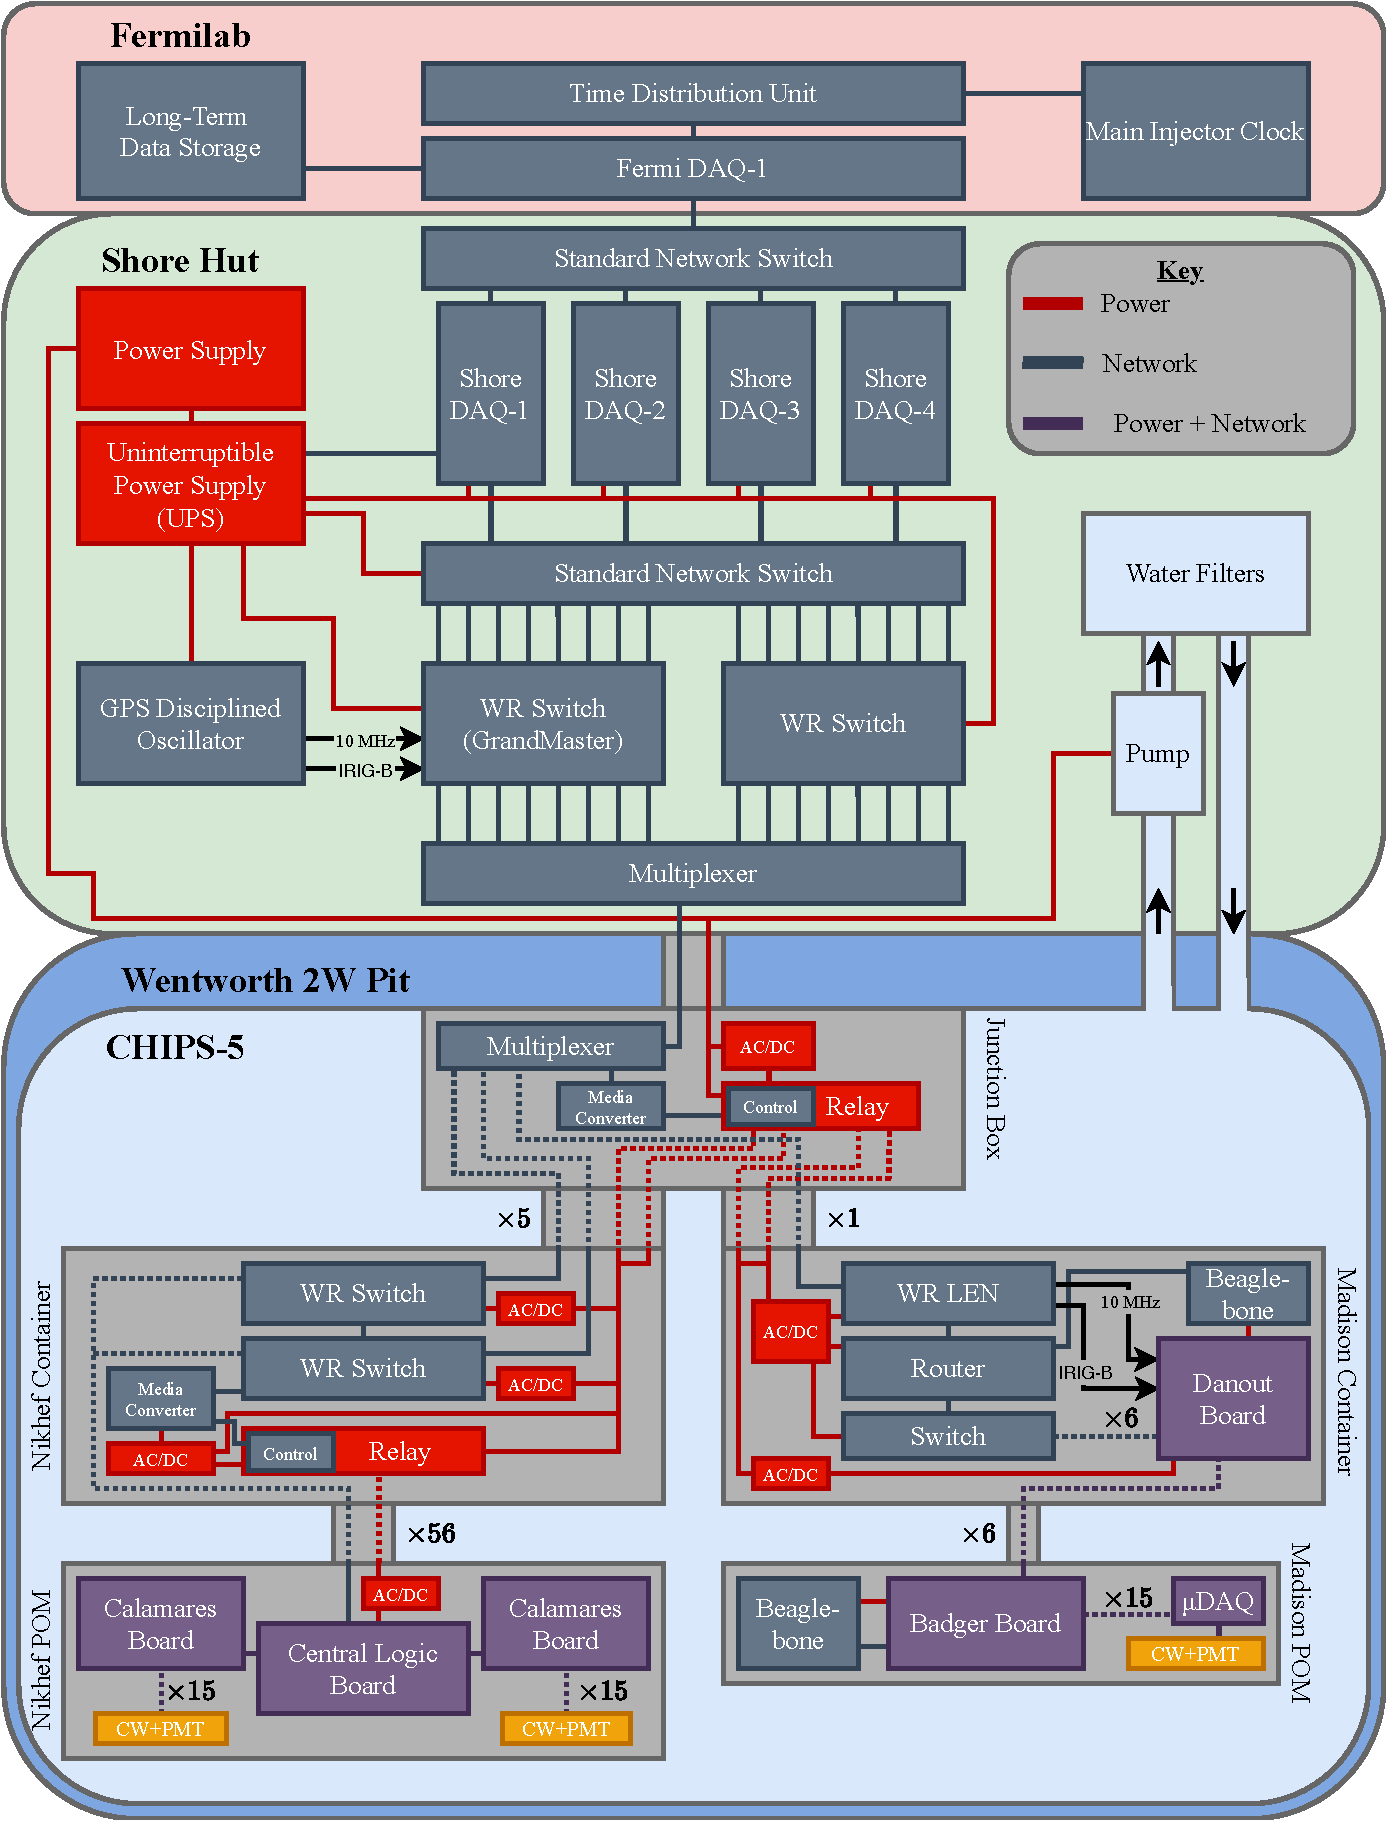
\includegraphics[width=\textwidth]{diagrams/5-daq/daq.pdf}
    \caption[Diagram of the \chipsfive data acquisition and power distribution system.]
    {Diagram of the \chipsfive DAQ and power distribution system.}
    \label{fig:daq}
\end{figure}

Common to both low-level hardware implementations is the use of the Time over Threshold (ToT)
method for PMT signal digitisation. Each analogue PMT pulse is fed to a ToT discriminator coupled
with a Time to Digital Converter (TDC) in order to generate a digitised recorded hit, as
illustratively shown in Fig.~\ref{fig:tot}. Even though ToT values are less accurate and do not
scale linearly with deposited charge, they are used instead of the more common Analogue to Digital
Converter (ADC) readout as the electronics are simpler and notably cheaper.

\begin{figure} % TOT DIAGRAM DIAGRAM %
    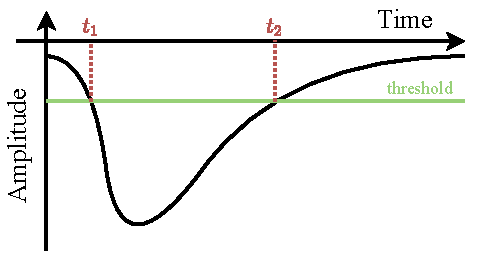
\includegraphics[width=0.6\textwidth]{diagrams/5-daq/tot.pdf}
    \caption[Illustrative diagram showing how Time over Threshold is measured.]
    {Illustrative diagram showing how a ToT value is measured. As soon as the rising edge of a PMT
        charge pulse rises above a given threshold (goes below in the negative charge case) a time
        is recorded $t_{1}$, when the falling edge later falls below the threshold a second time
        $t_{2}$ is recorded. The difference in time between $t_{1}$ and $t_{2}$ is output by the
        electronics as a digitised ToT value.}
    \label{fig:tot}
\end{figure}

\subsection{Nikhef hardware} %%%%%%%%%%%%%%%%%%%%%%%%%%%%%%%%%%%%%%%%%%%%%%%%%%%%%%%%%%%%%%%%%%%%%
\label{sec:daq_hard_Nikhed} %%%%%%%%%%%%%%%%%%%%%%%%%%%%%%%%%%%%%%%%%%%%%%%%%%%%%%%%%%%%%%%%%%%%%%

All Nikhef \unit{88}{\mathrm{mm}} HZC PMTs are attached directly to a simple readout board
containing a high-voltage generating Cockcroft-Walton circuit. Up to 30 PMTs are connected to two
\emph{Calamares} boards within the Nikhef POM electronics box via standard category 5 cables with
RJ45 connectors, as shown in Fig.~\ref{fig:nikhef_plane}. Both Calamares boards are directly
attached to a Central Logic Board (CLB)~\cite{biagi2015, eijk2015}. The CLB contains ToT
discriminators and TDCs to digitise the recorded PMT signals as well as electronics to synchronise
to the WR network clock for timestamping. Each Nikhef POM electronics box also contains an AC to
DC power converter whose output is fed into the CLB for distribution.

\begin{figure} % NIKHEF PLANE DIAGRAM %
    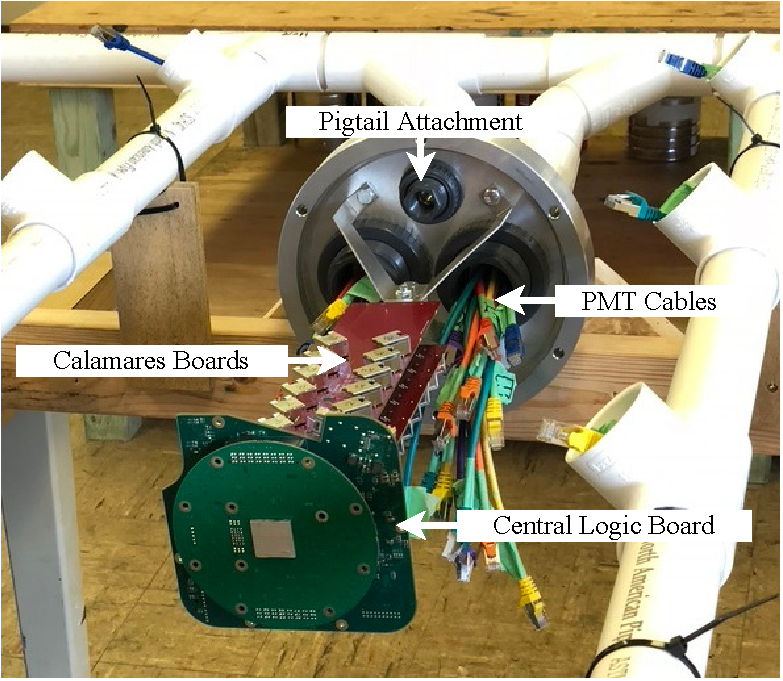
\includegraphics[width=0.8\textwidth]{diagrams/5-daq/nikhef_plane.pdf}
    \caption[Labelled picture of the Nikhef POM electronics box.]
    {Labelled picture of the Nikhef POM electronics box. Both ends of the PMT cables can be seen,
        either at the PMT mounting points, or entering the electronics box and not yet plugged
        into the Calamares boards.}
    \label{fig:nikhef_plane}
\end{figure}

Every Nikhef POM is connected via a single fibre and a power connection to a \emph{Nikhef
    container}, the contents of which are shown in the bottom half of Fig.~\ref{fig:full_setup}. A
total of five Nikhef containers are present within \chipsfive. Two WR switches are used within
each container to provide sufficient networking ports. Both are powered by independent AC to
DC converters and receive a single optical fibre connection each from the higher level DAQ
systems. An additional connection between each switch ensures that if one connection fails the
other can still be used to transfer data.

\begin{figure} % FULL SETUP DIAGRAM %
    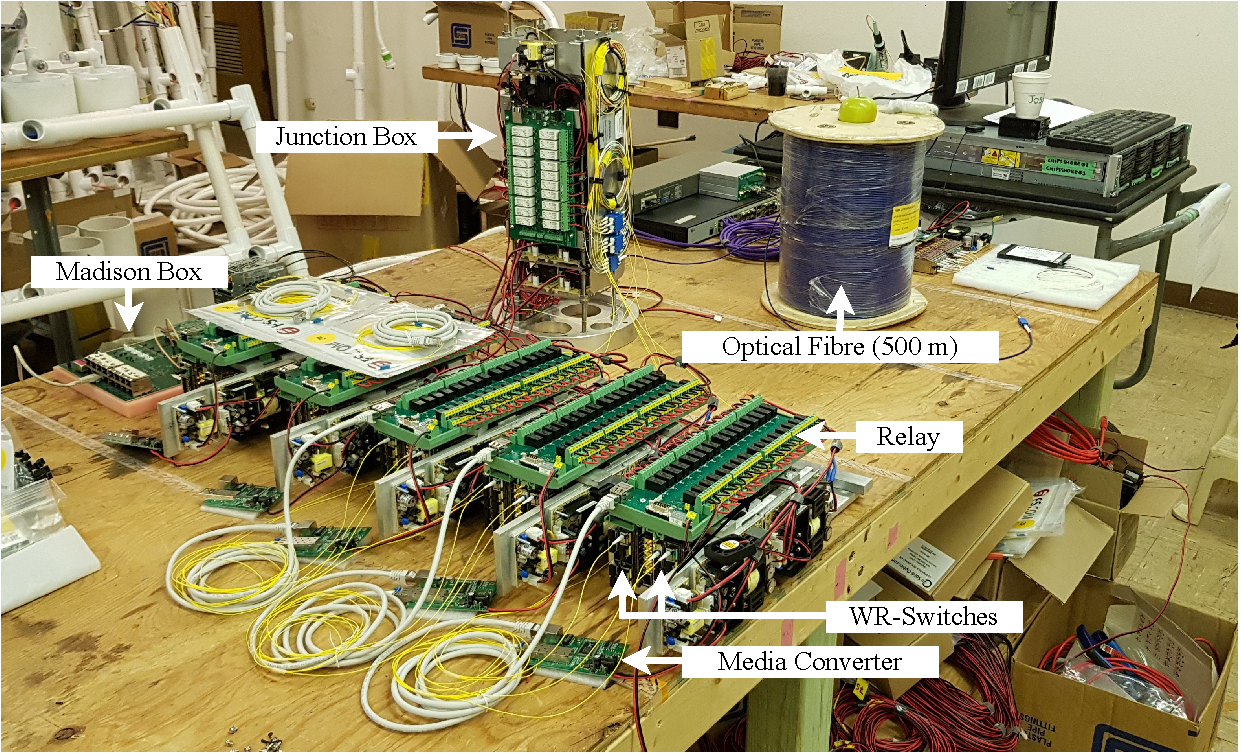
\includegraphics[width=\textwidth]{diagrams/5-daq/full_setup.pdf}
    %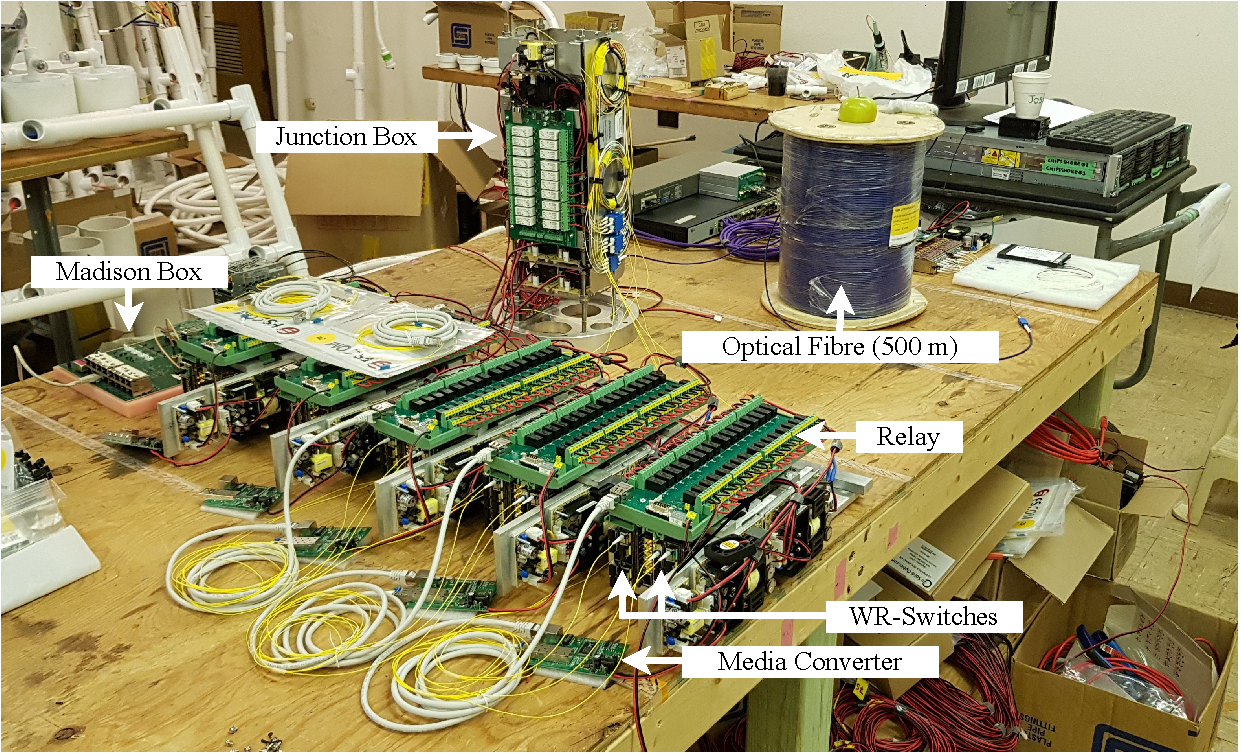
\includegraphics[angle=90,origin=c,width=0.8\textwidth]{diagrams/5-daq/full_setup.pdf}
    \caption[full set up short]
    {Picture of the full \chipsfive DAQ system}
    \label{fig:full_setup}
\end{figure}

Each container, contains two White Rabbit switches for networking (two to provide enough ports)
and a relay board for controlling the power to all attached POMs. A media converter converts a
fibre connection to a standard copper cable connection to control the relay, which is a network
device. Both switches are also reachable on the network mainly for monitoring. 2 ac/ds converters
provide power for each of the switches while a third powers the relay control electronics and
media converter. The relay outputs are connected directly to the input AC supply.

\subsection{Madison hardware} %%%%%%%%%%%%%%%%%%%%%%%%%%%%%%%%%%%%%%%%%%%%%%%%%%%%%%%%%%%%%%%%%%%%
\label{sec:daq_hard_madison} %%%%%%%%%%%%%%%%%%%%%%%%%%%%%%%%%%%%%%%%%%%%%%%%%%%%%%%%%%%%%%%%%%%%%

Every Madison Hamamatsu R6091 PMT is directly attached to a high-voltage generating
Cockcroft-Walton board followed by a signal processing \emph{$\mu$DAQ}, as shown in
Fig.~\ref{fig:madison_pmt_assembly}. The $\mu$DAQ is a small microcontroller developed for both
the IceCube experiment and \chips at WIPAC in Madison. Capable of timestamping and digitising
signals directly at the PMT level, the $\mu$DAQ also sets the PMT operating voltage by controlling
the Cockcroft-Walton board~\cite{eijk2018}.

Up to 16 $\mu$DAQs receive power, networking, and PPS and \unit{10}{\mathrm{MHz}} timing signals
from a \emph{badger-board}, as shown in Fig.~\ref{fig:madison_plane}. Standard category 5 cables
with RJ45 connectors are used. The badger-board is located within the electronics box of each
Madison POM and acts as a simple fanout and power control board. For logic, each badger-board has
an attached mezzanine Beaglebone~\cite{beagle2020}. This single-board Linux machine (very similar
to a Raspberry Pi) controls the power supply to and receives hits from the attached $\mu$DAQs.

\begin{figure} % MADISON PLANE DIAGRAM %
    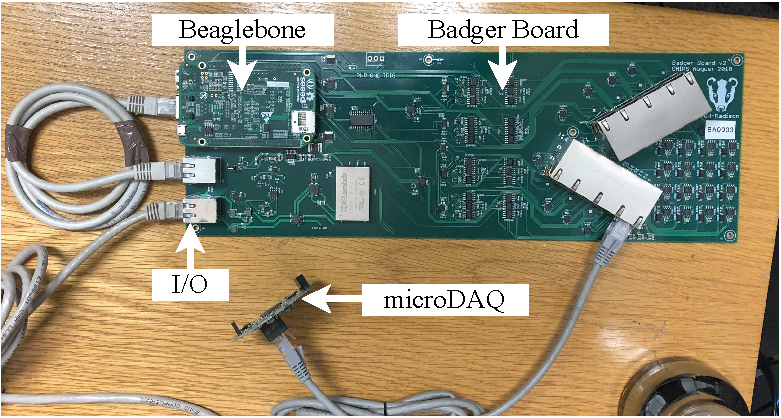
\includegraphics[width=0.8\textwidth]{diagrams/5-daq/madison_plane.pdf}
    \caption[Labelled picture of the components of the Madison POM electronics box.]
    {Labelled picture of the components of the Madison POM electronics box.}
    \label{fig:madison_plane}
\end{figure}

Similarly up to 16 Madison POM badger-boards receive power, networking and PPS and
\unit{10}{\mathrm{MHz}} timing signals from a \emph{danout-board} located within a single
\emph{Madison container}. Again, standard category 5 cables with RJ45 connectors are used. The
full contents of the Madison container are shown in Fig.~\ref{fig:madison_box}. Similar to the
badger-board, the danout-board acts as a simple fanout and power control board with an attached
mezzanine Beaglebone. However, in this case, the attached Beaglebone acts just to control the
power provided by the danout-board.

PMT hits and other packets are instead routed straight through the danout-board into a networking
stack. Consisting of a WR LEN, a router (required due to the limited WR LEN routing table size),
and a switch, the stack provides network connections to the higher-level DAQ via a single optical
fibre and synchronisation with the WR clock. The synchronised PPS and \unit{10}{\mathrm{MHz}}
timing signals are taken as an output from the WR LEN and sent to the danout-board for forwarding
to the lower-level components. Additionally, two AC to DC converters provide power for the devices
within the container and all lower-level components through connections with the danout-board.

\begin{figure} % MADISON BOX DIAGRAM %
    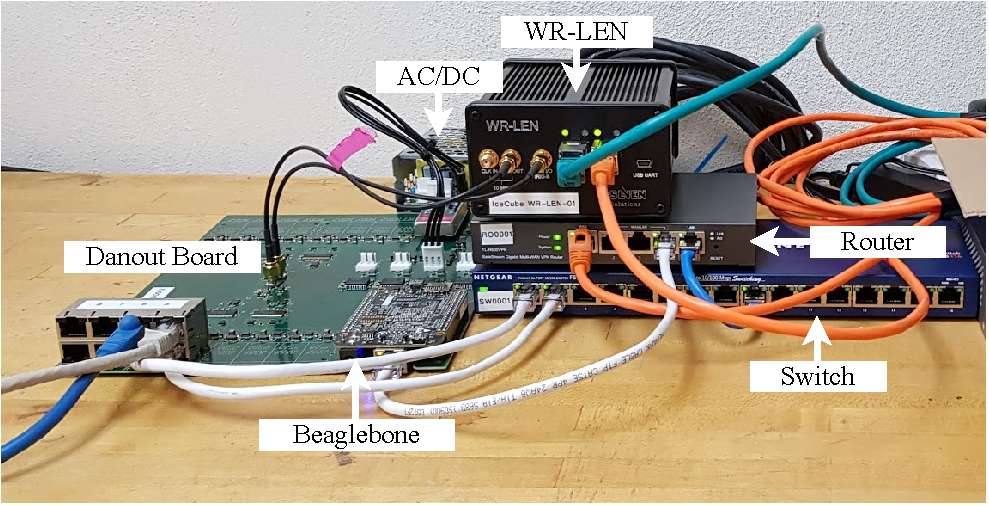
\includegraphics[width=\textwidth]{diagrams/5-daq/madison_box.pdf}
    \caption[Labelled picture of the Madison container components.]
    {Labelled picture of the Madison container components. The blue and grey cables exiting the
        left hand side of the image go to individual Madison POMs connecting to the I/O port shown
        in fig.~\ref{fig:madison_plane}. An optical fibre connection into the left SFP port of the
        WR LEN is used in reality rather than the copper connection shown here.}
    \label{fig:madison_box}
\end{figure}

- Can reference the Nikhef stuff that I have already described - THIS IS WHAT ALL FUTURE CHIPS
DETECTOR SHOULD USE FULLY!!! - This is the novel stuff that is much cheaper! NOVEL NOVEL NOVEL
CHEAP CHEAP CHEAP SIMPLE SIMPLE SIMPLE COMMERCIAL COMMERCIAL COMMERCIAL CAPABLE CAPABLE CAPABLE
LINUX LINUX LINUX Can configure at a later data as we have a full linux machine at a very low
level of the DAQ system. Can do lots of processing close to where the DAQ inputs are created.
unlike in the Nikhef case where it is done on the CLB. As the beaglebone is a full linux machine
at a low level lots of processing can occur close to the PMTs. It controls the power and
networking on the $\mu$DAQ, receives their hits before forwarding further up the chain. The
$\mu$DAQ and beaglebone are novel approaches, CHEAP, more processing close to PMTs!!! commercially
available!!

\subsection{Combined systems} %%%%%%%%%%%%%%%%%%%%%%%%%%%%%%%%%%%%%%%%%%%%%%%%%%%%%%%%%%%%%%%%%%%%
\label{sec:daq_hard_combined} %%%%%%%%%%%%%%%%%%%%%%%%%%%%%%%%%%%%%%%%%%%%%%%%%%%%%%%%%%%%%%%%%%%%

- Multiplexer allows for 16 different channels using wavelengths between 1310nm and 1550nm with
corresponding SFPs (Small Form-Factor Pluggable Transceiver)

The Junction box contains connections to each container and their power supply relays. The two
input power connections from shore are distributed to via two copper plates to all the relay
connections throughout the box. Two standard network controlled logic relays control "trip" gates
that stop the power supply to any/ section of the detector is a power surge is detected. THis is
especially important for CHIPS given the water that is everywhere :p. One relay controls a pulsing
and one just opens the channels. The trip gates are opening via a short pulse of current. Tye
multiplexer contains 18 channels each a different wavelength of light allowing a huge volume of
data to be sent up a single fibre to shore. Each WR switch or WR LEN in the madison case has the
corresponding receiver SFP as the ones o shore.

Within the shore hut all networking comes in through the multiplexer and is split back out into its
individual wavelength channels via the multiplexer these go into multiple ports on two white
rabbit switches. This is mainly for data flow such that each can be segmented via a VLAN with the
corresponding ports on the opposite side and then the higher level standard networking switch to
provide DO THE CALCULATION HERE lots of data bandwidth up to the main DAQ machines. One of the WR
switches is the GrandMaster for the WR network and receives the PPS and 10MhZ input from the GPs
disciplines oscillator which is connected to a GPS antenna to receive its signals. Again both
switches are also on the DAQ network for monitoring and control.

The standard switch acts as the switch for condensing traffic onto single 10Gb connections to each
individual DAQ machine. This is also on the network via a control port for monitoring. Only a
single DAQ machine is used for data taking which another is used for monitoring and control as
detailed in Section... The standard network switch is also connected to the wider CHIPS network at
the pit the polymet building and then the wider internet for data transfer to fermilab!

\begin{figure} % MANIFOLD DIAGRAM %
    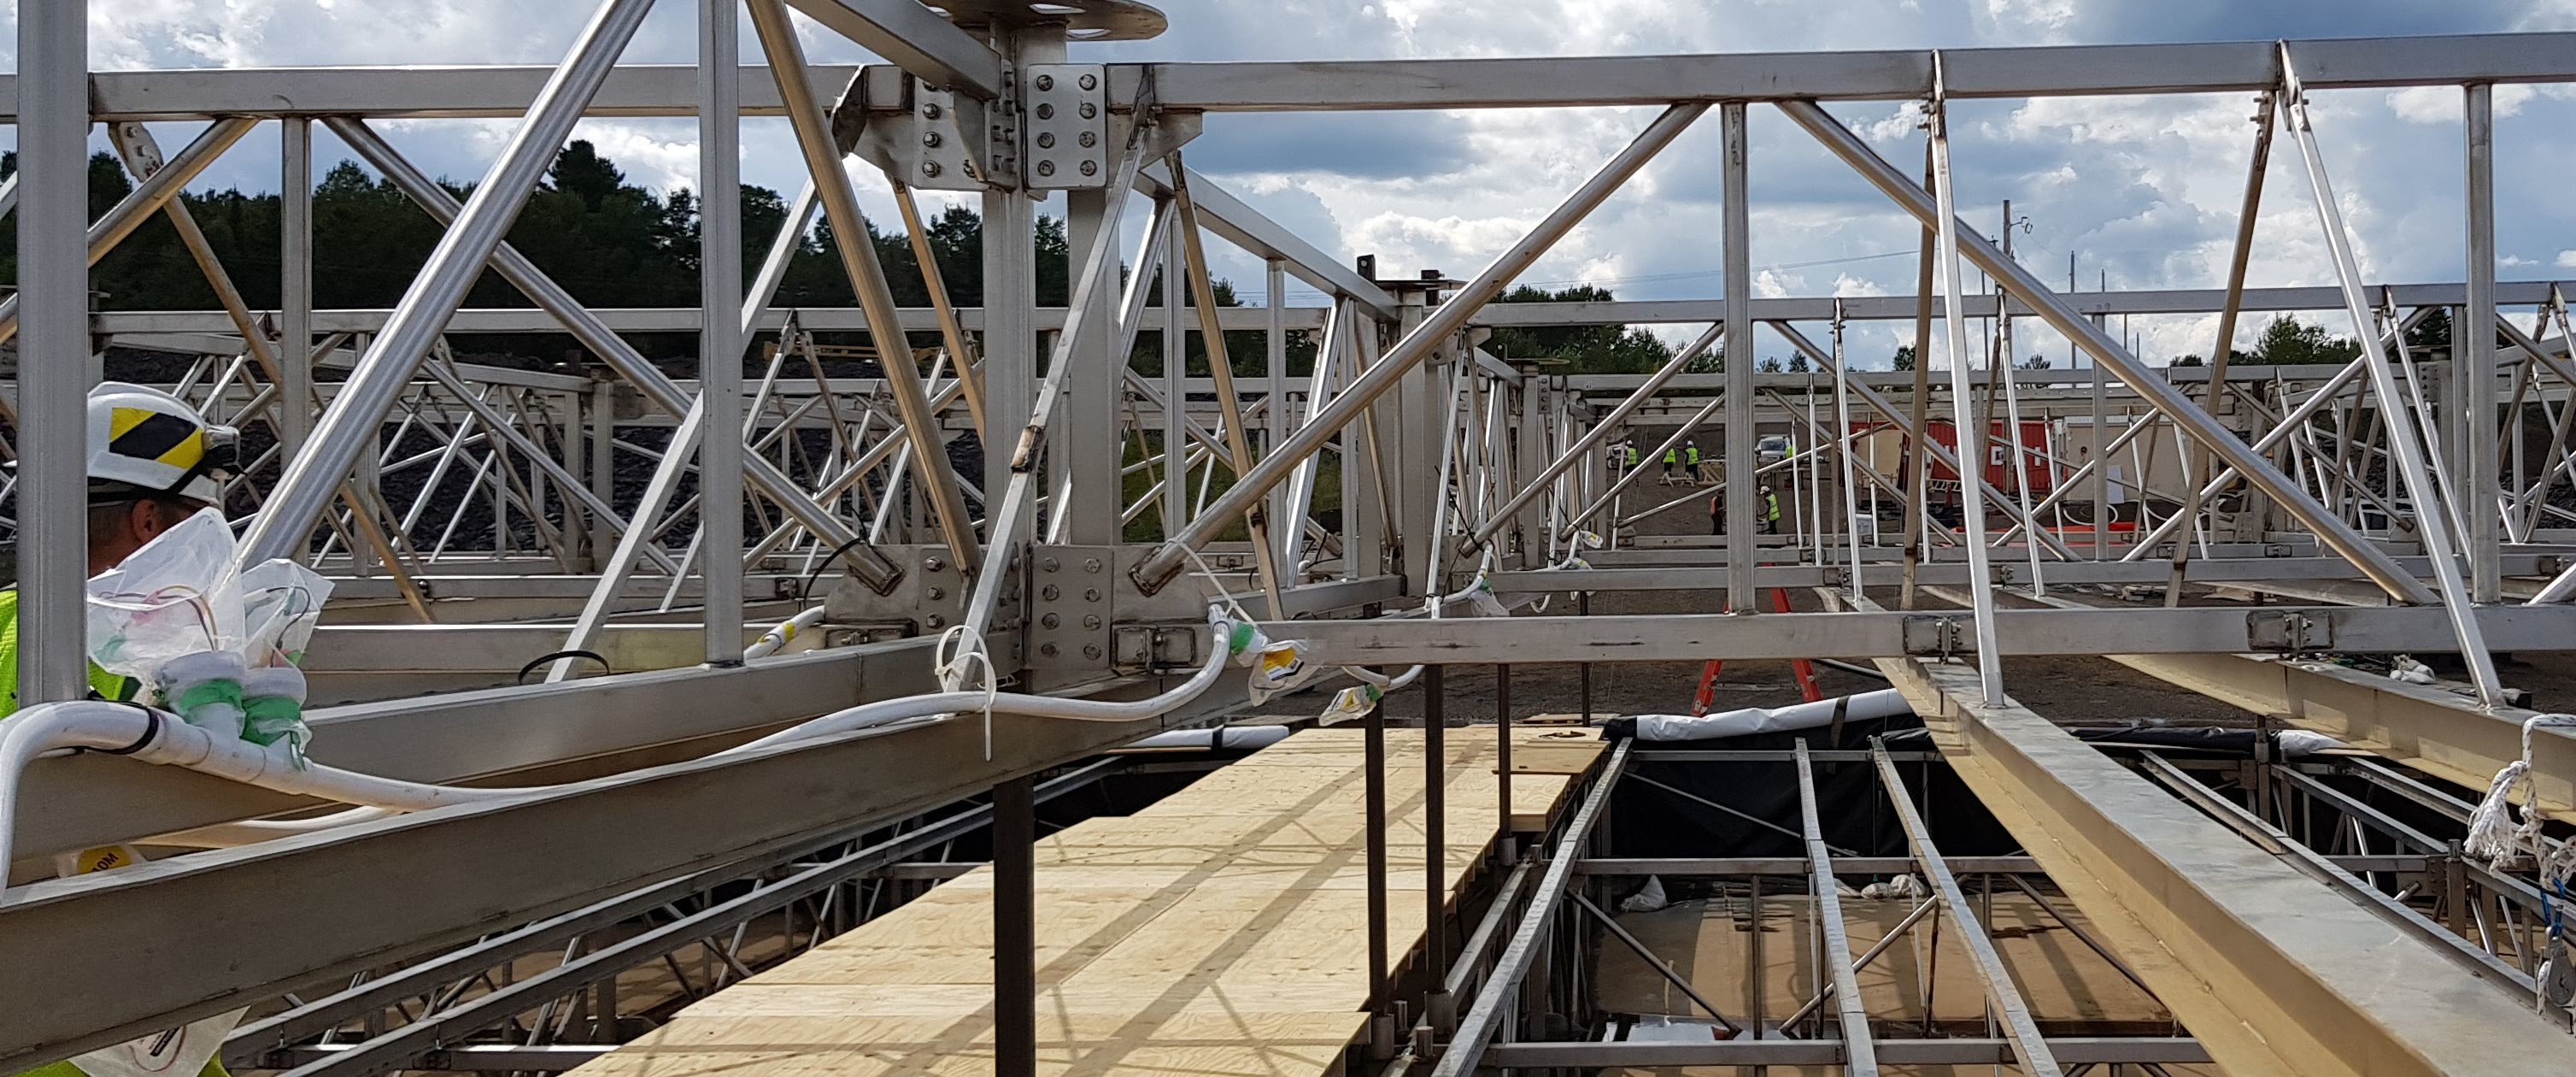
\includegraphics[width=\textwidth]{diagrams/5-daq/manifold.jpg}
    \caption[manifold short]
    {manifold long}
    \label{fig:manifold}
\end{figure}

\begin{figure} % WHITE-RABBIT GM SETUP DIAGRAM %
    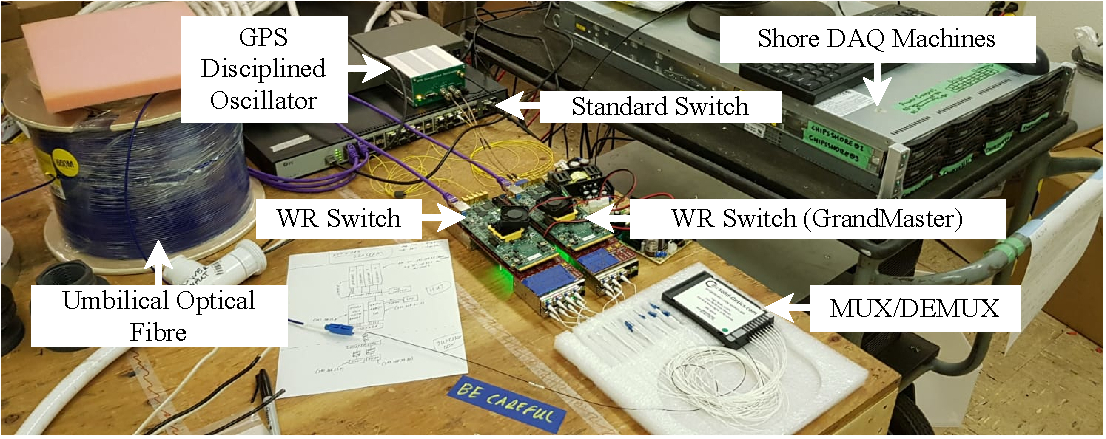
\includegraphics[width=\textwidth]{diagrams/5-daq/hut_daq.pdf}
    \caption[hut daq short]
    {hut daq long}
    \label{fig:hut_daq}
\end{figure}

\section{Software} %%%%%%%%%%%%%%%%%%%%%%%%%%%%%%%%%%%%%%%%%%%%%%%%%%%%%%%%%%%%%%%%%%%%%%%%%%%%%%%
\label{sec:daq_soft} %%%%%%%%%%%%%%%%%%%%%%%%%%%%%%%%%%%%%%%%%%%%%%%%%%%%%%%%%%%%%%%%%%%%%%%%%%%%%

TODO: Write the software section of the DAQ chapter

~\cite{chipsdaq2020}

- What makes this implementation special
- Limited resource, but brilliant capabilities
- Use existing software when possible

- Need to talk about what is novel, new and exciting!
- Not so much about the hardcore electronics details, more high level
- FINITE STATE MACHINE!!!

SOFTWARE
- The beam spill
- Hit acquisition and handling
- Detector and data quality monitoring

\begin{figure} % SOFTWARE DIAGRAM %
    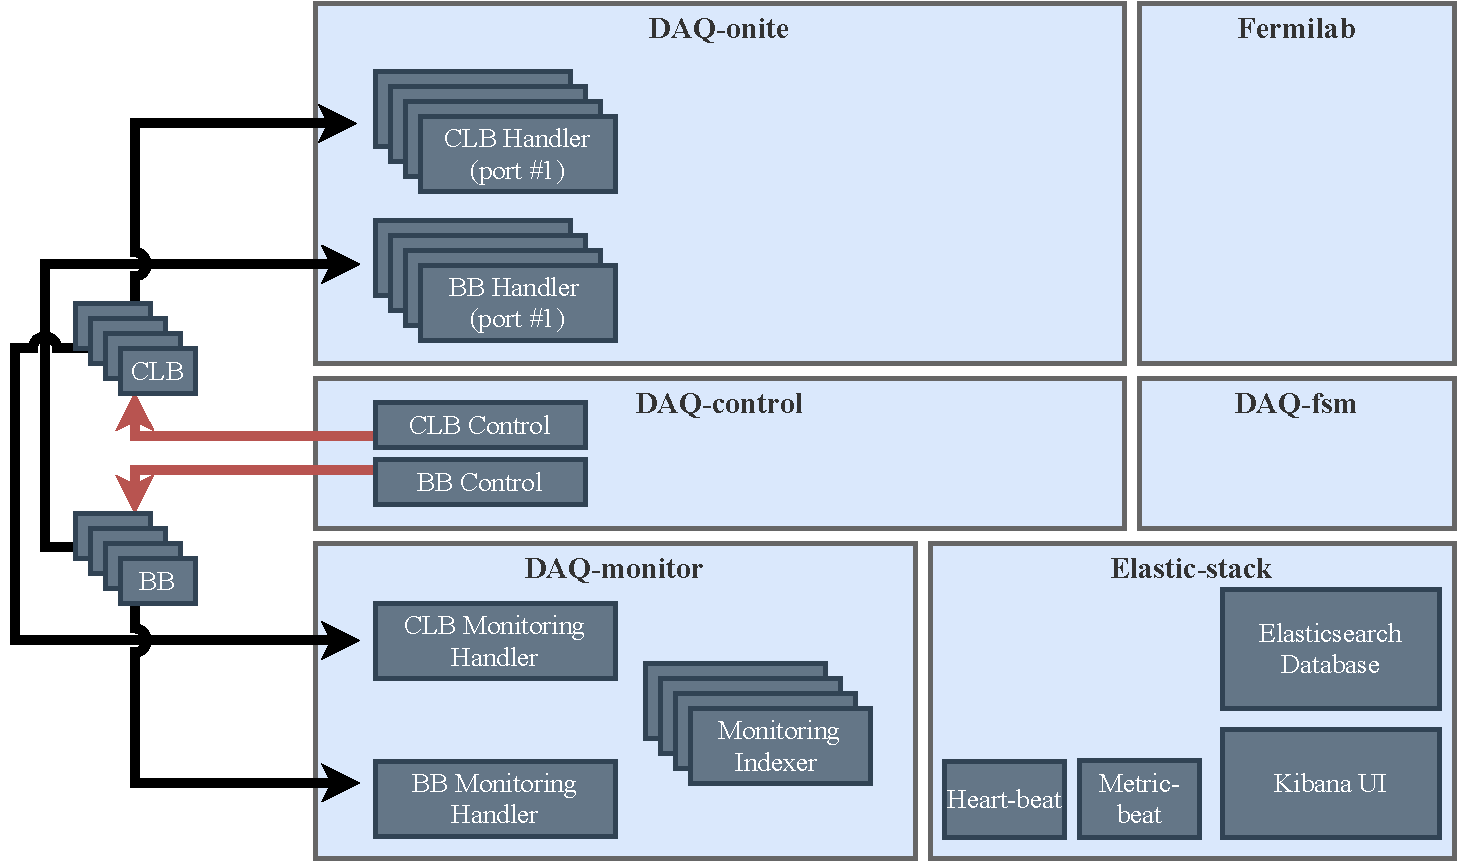
\includegraphics[width=\textwidth]{diagrams/5-daq/daq_software.pdf}
    \caption[daq software short]
    {daq software long}
    \label{fig:daq_software}
\end{figure}

- INCLUDE DATA RATES IN SOFTWARE DIAGRAM
- INCLUDE WHICH MACHINES THINGS RUN ON IN SOFTWARE DIAGRAM

- Separated into slow-control, data collection, and

- Need to get across what makes this DAQ implementation special and novel, what are the
interesting unique bits of it? Limited resources but great performance! Use of existing hardware
and software! Modern approaches to doing things, good part of small collaboration!
- Needs to able to cope with 4 degrees at bottom!
- Talk about expected data through put, what we can cope with
- Jumbo frames etc

- An `all-data-to-shore' approach as done in KM3NeT
- Data is sent in UDP packets (not TCP so some will go missing)
- $\mu$DAQ software repository with fh-library (field-hub) novel communication library
in~\cite{microdaq2020}. Most of Madison code is written in c!
- Mainly written in C++, full asynchronous using the BOOST Asio library in~\cite{boost2020} which
is a library for network and low-level I/O programming using an asynchronous model.
- Taking inspiration from the KM3NeT DAQ Java software
- The detector is configured using a single human readable configuration file that defines all the
POM types, MAC addresses, IP addresses, types, relay channels, which channels should be active and
their associate high voltage setting, threshold and electronic ID.
- Typical ethernet frame has a maximum transmission unit (MTU) size of 1500 bytes, we use Jumbo
frames that allow for an MTU of 9000 bytes, this means we have a lot less small frames with only a
limited number of recorded hits, which proved to be taxing to the switches and lead to an increase
in the number of dropped frames.
- 1Gb links between WR switches, 10Gb link between FS switch and main DAQ machine. Provides
sufficient bandwidth, DO A SMALL CALCULATION!

\subsection{The beam spill} %%%%%%%%%%%%%%%%%%%%%%%%%%%%%%%%%%%%%%%%%%%%%%%%%%%%%%%%%%%%%%%%%%%%%%
\label{sec:daq_soft_spill} %%%%%%%%%%%%%%%%%%%%%%%%%%%%%%%%%%%%%%%%%%%%%%%%%%%%%%%%%%%%%%%%%%%%%%%

\subsection{Hit acquisition and handling} %%%%%%%%%%%%%%%%%%%%%%%%%%%%%%%%%%%%%%%%%%%%%%%%%%%%%%%%
\label{sec:daq_soft_hits} %%%%%%%%%%%%%%%%%%%%%%%%%%%%%%%%%%%%%%%%%%%%%%%%%%%%%%%%%%%%%%%%%%%%%%%%

\subsection{Detector and data quality monitoring} %%%%%%%%%%%%%%%%%%%%%%%%%%%%%%%%%%%%%%%%%%%%%%%%
\label{sec:daq_soft_monitor} %%%%%%%%%%%%%%%%%%%%%%%%%%%%%%%%%%%%%%%%%%%%%%%%%%%%%%%%%%%%%%%%%%%%%

- Elasticsearch ref in~\cite{elastic2020}
- An open source RESTful, JSON-based, search engine and noSQL database.
- Data is stored in \emph{indices} in individual \emph{documents}
- Get to leverage an enormous amount of online support and the community
- daqlog: Uses for DAQ application logging with a severity
- daqstate: Used to report the current state of various DAQ applications
- monpom: Used for reporting general POM monitoring information, such as temp, humidity, status
- monchannel: Used for reporting individual channel monitoring, such as rate, veto
- A series of altering rules are also set up constantly monitoring the status of the monitoring
data contained within the elasticsearch database to alert via slack or email individuals if something goes wrong.
- We index asynchronously to not block data taking, all data is backed up easily.
- Use the Kibana user interface which is accessible through a browser, means that no special
equipment, or GUIs are used, anyone on any machine has access to the full monitoring stack from
their browser. A series of dashboards ar set up to monitor everything within the detector.
- A series of indices are set up to store data which is sent via standard REST messages to the
database, the special indexing allows for quick `searching' over any time period etc... for
monitoring.
- Also means that anyone can quickly/easily look at any part of the data and make plots etc...
without needing to write an additional part of a monitoring program.

\begin{figure} % MONITORING DIAGRAM %
    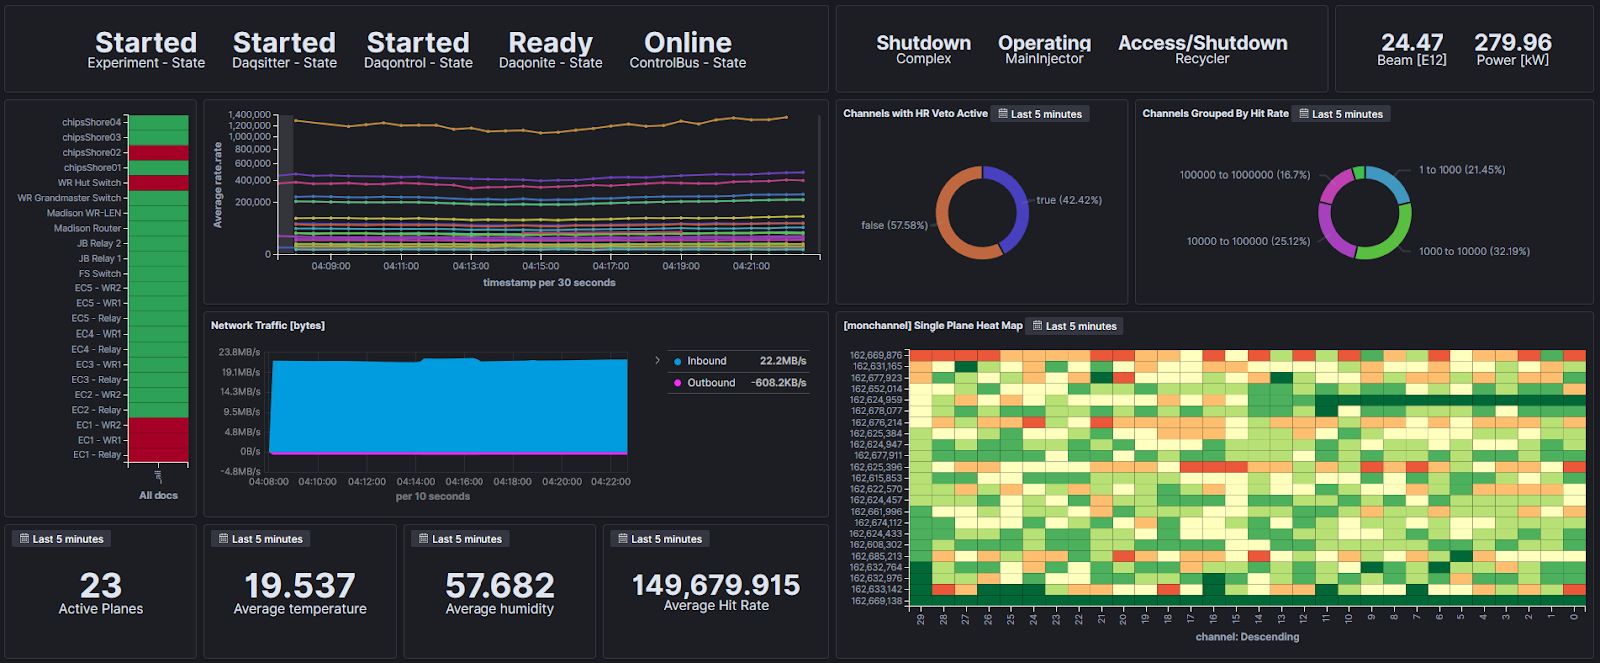
\includegraphics[width=\textwidth]{diagrams/5-daq/monitoring.png}
    \caption[monitoring short]
    {monitoring long}
    \label{fig:monitoring}
\end{figure}